\documentclass[letterpaper]{article}
\usepackage{amsmath}
\usepackage{algorithm}
\usepackage{multirow}
\usepackage{graphicx}

\DeclareMathOperator*{\argmin}{arg\,min}

\begin{document}
\title{ECON 199 Problem Set 1}
\author{Will Koster (jameswk2)}
\author{Javier Garza (javierg2)}
\date{Feb 25, 2020}
\maketitle

\clearpage

\section{Problem 1}
\begin{enumerate}
    \item 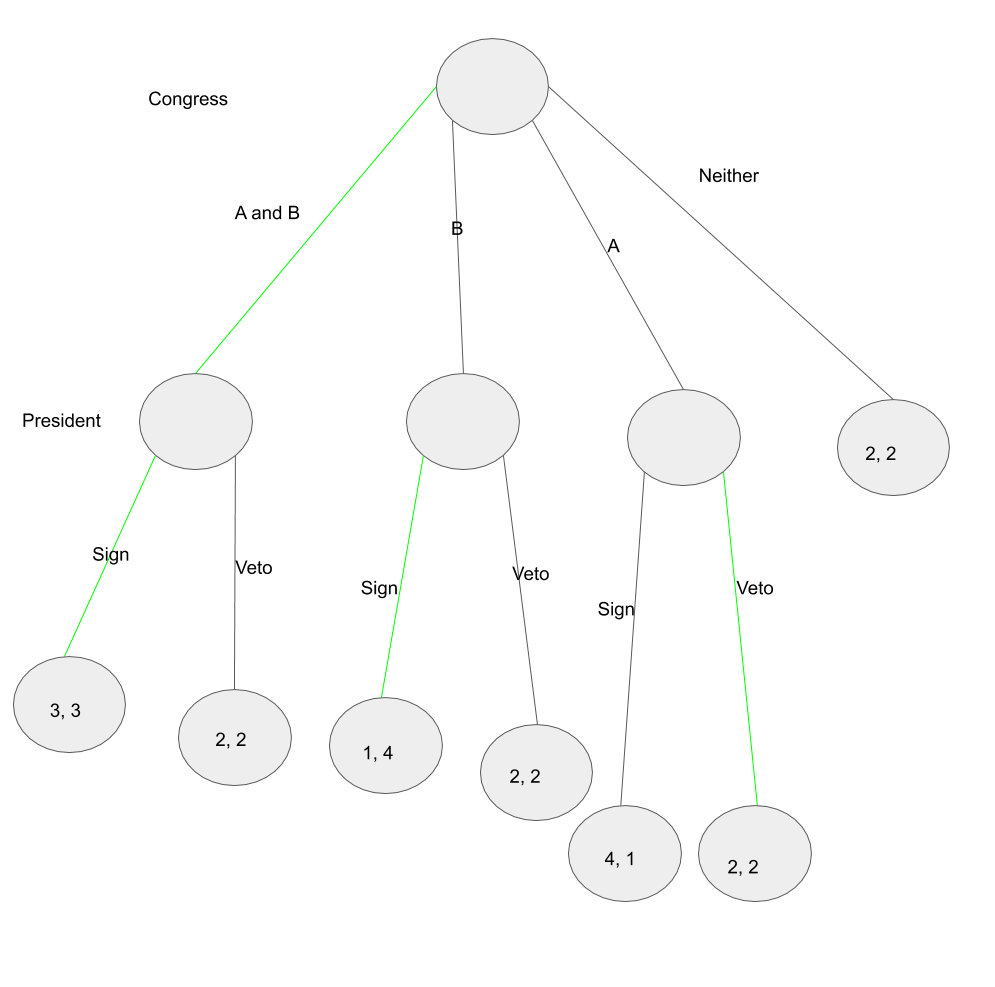
\includegraphics[scale=0.4]{fig1}
    \item 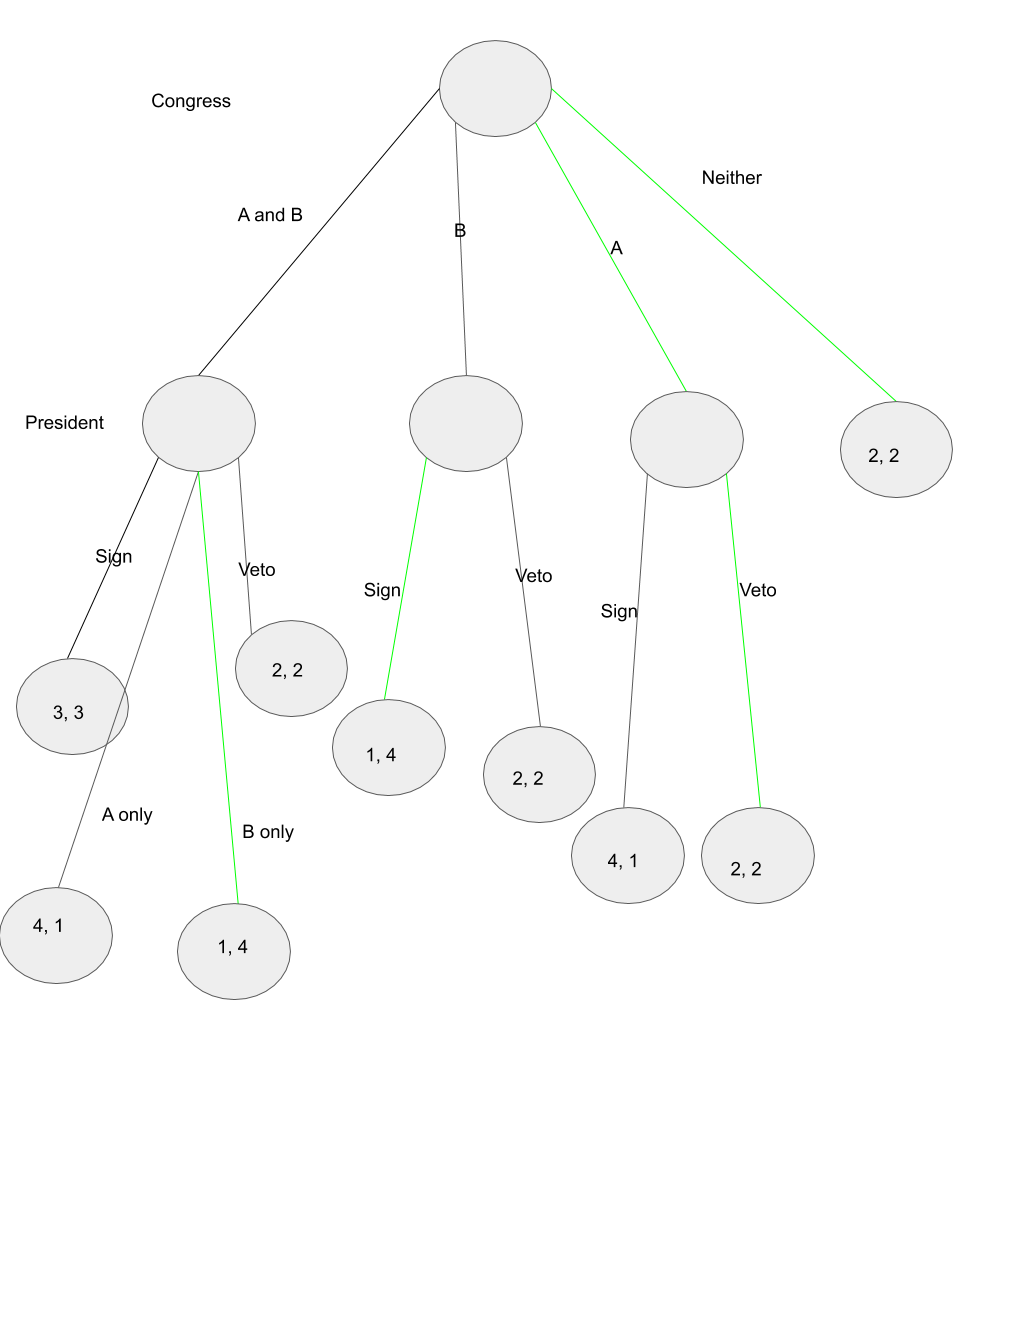
\includegraphics[scale=0.4]{fig2}
    \item In the first situation, Congress could force the President to give it something in exchange for giving the President what he wanted, but in the second situation, that was no longer the case, so Congress no longer had any incentive to give the President anything.
\end{enumerate}

\section{Problem 2}
\begin{enumerate}
    \item 
David Buys \\
\begin{tabular}{|l|l|l|l|}
\multicolumn{4}{c}{Colleen}                      \\ \hline
\multirow{3}{*}{Bruce} &   & B        & N        \\ \hline
                       & B & $10,10,10$ & $\overline{10},\overline{20},\overline{10}$ \\ \hline
                       & N & $\overline{20},\overline{10},\overline{10}$ & $0,0,-10$ \\ \hline
\end{tabular} \\
David does not buy \\
\begin{tabular}{|l|l|l|l|}
\multicolumn{4}{c}{Colleen}                      \\ \hline
\multirow{3}{*}{Bruce} &   & B        & N        \\ \hline
                       & B & $\overline{10},\overline{10},\overline{20}$ & $-10,0,0$  \\ \hline
                       & N & $0,-10,0$ & $\overline{0},\overline{0},\overline{0}$ \\ \hline
\end{tabular}\\

\item The Nash equilibria are when any two people buy sushi or none of them do.  
\item Unless there were some situation that is not captured in the game (eg David lives next door to the sushi place, Colleen is the wealthiest, etc), we would have to assume that every member of the group makes the same independent decision. In that case, the focal point would likely be that no one buys sushi, since, under the assumption that your friends do the same thing, it's always optimal for you to not buy sushi, regardless of what they both choose to do.
\end{enumerate}
\section{Problem 3}
\begin{enumerate}
    \item If we assume that everyone is equally rational and that they will all come to the same conclusion, the symmetric Nash equilibrium will be $\argmin_x |x - \left(\frac{2}{3}(x + 9)\right)| = 18$. No individual can improve their own outcome by unilaterally changing their number, which guarantees that this is a Nash equilibrium.
    \item The lowest possible best number is $6$, which comes if everyone plays $0$. All the other possible best numbers are higher, which means that $6$ will be better than $5$ no matter what happens.
    \item $72\frac{2}{3}$ is the highest possible best number, which comes if the mean is $100$. $89$ is therefore closer to every possible best number than $90$, making $90$ a dominated strategy.
    \item Numbers greater than $72$ or less than $6$ are strictly dominated, since the best number will always be closer to another integer than to any of those numbers. 
    \item Since her classmates will never pick numbers below $6$ or greater than $72$, Elsa should never pick numbers less than $10$, the smallest best number that can arise if numbers less than $5$ are not chosen, or greater than $54$, the largest best number that can arise if numbers greater than $72$ are not chosen.
    \item Since this is a symmetric game and all players are equally rational, it's resonable to imagine that all the other players function as a single entity, since they are all rational and will come to the same conclusion. That gives you a 2-dimensional payoff matrix, which has only one Nash equilibrium, at (18, 18). Therefore, this is the most rationalizable outcome. In some sense, however, every strategy that isn't a best response to a dominated strategy (ie, any number between $10$ and $54$) is rationalizable.
        
\end{enumerate}

\end{document}
